
\newcommand{\pd}[2]{\frac{\partial{#1}}{\partial{#2}}}
\newcommand{\pdd}[2]{\frac{\partial^2{#1}}{\partial{#2}^2}}

\documentclass[a4paper]{report}

\usepackage[tmargin=1in,bmargin=1in,lmargin=0.75in,rmargin=0.75in]{geometry}

\linespread{1.5}
\usepackage{fancyhdr}
\usepackage{lipsum}
\usepackage{mathtools}
\usepackage{tikz}
\usepackage{pgfplots}
\usepackage{amsmath}
\usepackage[most]{tcolorbox}
\begin{document}

\pagestyle{fancy} % Set the page style to fancy

\fancyhf{} % Clear all header and footer fields
\fancyhead[L]{\includegraphics[width=1.0in]{logo.png}} % Left header
\fancyhead[C]{} % Center header (empty)
\fancyhead[R]{} % Right header (empty)
\fancyfoot[C]{\thepage} % Page number in the center footer

\begin{titlepage}
    \begin{center}
        \vspace*{1cm}
            
        \Huge
        \textbf{Maths and Statistics for AI and Data Science}
            
        \vspace{0.5cm}
        \LARGE
        Practical Assessment – 2
            
        \vspace{1.5cm}
            
        \textbf{by Uttara Naidu}
            
        \vfill
            
        Submitted to            

        The University of Liverpool\\

        26/05/2025
            
    \end{center}
\end{titlepage}     


\lhead[LO,LE]{\includegraphics[width=1.3in]{logo.png}}
%\fancyhead[LO,LE]{}

\section*{Question 1}

1. Out of 120 students in a school, 30 play rugby, 20 play badminton, and 5 play both sports.

a. How many students play neither sport? 

b. What is the probability that a randomly chosen student plays badminton? 

c. Given that a chosen student plays rugby, what is the probability that they also play badminton? 
\newline 2. Box 1 contains 6 red beans and 4 green beans. Box 2 contains 5 red beans and 3 green beans. A fair six-sided die is thrown. If a ‘2’ is obtained, a bean is selected from box 1; otherwise, a bean is selected from box 2. Given that the bean selected was red, what is the probability that it came from box 1? 
\newline 3. The probability that a student is late for a lesson is 0.1, independently of any other students. What is the probability that at least one of 10 students in a class is late? 

\textit{Provide appropriate justification and explanation to all your answers, detailing the methods used.}

\subsection*{Solution:}

\subsubsection*{1.a) Find  number of students who play neither Badminton nor Rugby}

\paragraph{}


\begin{center}
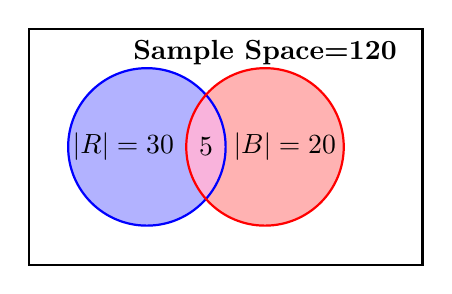
\begin{tikzpicture}
     % Define colors for the circles
    \begin{scope}
        % Left Circle (circle A)
        \fill[blue!30] (0,0) circle (1);
        % Right Circle (circle B)
        \fill[red!30] (1.5,0) circle (1);
    \end{scope}

    % Intersection Circle
    \begin{scope}
        \clip (0,0) circle (1);
        \fill[magenta!30] (1.5,0) circle (1);  % Change the color here
    \end{scope}
    % Label circles
    \node at (-0.3, 0) {\textbf{$|R|=30$}};
    \node at (1.75, 0) {\textbf{$|B|=20$}};

    % Intersection text
    \node at (0.75, 0) {5};
    % Draw the outlines for clarity
    \draw[blue, thick] (0,0) circle (1);
    \draw[red, thick] (1.5,0) circle (1);
    % Sample space rectangle
    \draw[thick] (-1.5,-1.5) rectangle (3.5,1.5);
    \node at (1.5, 1.2) {\textbf{Sample Space=120}};  % Positioned inside the rectangle, at the top

\end{tikzpicture}
\end{center}


The above Venn diagram represents the given population. 

Let the number of students playing Rugby be represented as $|R|$ and for Badminton be represented as $|B|$.

\begin{align*}
|R|&=30 \\
|B|&=20 \\
|R \cap B|&=5 
\end{align*}


As per the principle of Inclusion-Exclusion (ACP,2024), we get the number of active sports players as,



\begin{align}
    \notag|R\cup B|&=|R|+|B|-|R\cap B| \\
    \notag&=30+20-5\\
    |R\cup B|&=45
\end{align}

Hence the total number of students who play either Rugby or Badminton or both is $45$.

We have the sample space $|S|$ (or universal set) of size $120$. Calculating the total number of students $|T|$ playing neither sport as below,

\begin{align*}
    |T|&=|S|-|R\cup B| \\
    &=120-45
\end{align*}

\begin{equation}
  \boxed{|T|=75}
\end{equation}


\subsubsection*{1.b) Find  the probability that a randomly chosen student plays badminton}

\paragraph{}

Since the problem statement asks for a "randomly chosen student" (and not "only the students playing sports"), we consider the entire sample space of $120$.

Hence, the probability $P(B)$ that a randomly chosen student plays Badminton is given by,

\begin{align*}
    P(B)&=\frac{number\ of\ students\ playing\ Badminton}{total\ student\ population} \\
    &=\frac{20}{120}\\
    &=0.1667
\end{align*}

\begin{equation}
    \boxed{P(B) \approx 16.67\%}
\end{equation}


\subsubsection*{1.c) Find  the probability that a chosen student plays Badminton given that they play Rugby}

\paragraph{}

Given the occurence of event $B$, the probability of event $A$ occuring is given by below formula (UoL,2025):

\begin{equation}
    \color{blue} P(A|B)=\frac{P(A\cap B)}{P(B)} \tag{A}
\end{equation}

This is called conditional probability.

For the problem statement, let us state the below terms:

$P(R)$ is probability of a chosen student who plays Rugby.

$P(B)$ is probability of a chosen student who plays Badminton.

$P(B\cap R)$ is probability of chosen student who plays both Rugby and Badminton

Using these terms in formula $(A)$, we get,

\begin{align}
    P(B|R)=\frac{P(B\cap R)}{P(R)}
\end{align}

where $P(B|R)$ is the probability that a student plays Badminton given that they play Rugby.

From equation $(1)$, let us consider a sub-sample space of student population of $\color{blue}45$ i.e. only the students who are active in sports.

\subparagraph{Step i: Calculating $P(B\cap R)$}


\begin{align}
    \notag P(B\cap R) &= \frac{number\ of\ students\ playing\ Rugby\ and Badminton}{|R\cup B|} \\
    \notag &=\frac{|B\cap R|}{45} \\
    \notag &=\frac{5}{45} \\
    P(B\cap R) &= \frac{1}{9}
\end{align}


\subparagraph{Step ii: Calculating $P(R)$}

\begin{align}
    \notag P(R)&=\frac{number\ of\ students\ playing\ Rugby}{|R\cup B|} \\
    \notag &=\frac{30}{45} \\
    P(R)&=\frac{2}{3}
\end{align}


Subsctituting $(5)$ and $(6)$ into $(4)$, we get,

\begin{align*}
    P(B|R)&=\frac{\frac{1}{9}}{\frac{2}{3}} \\
    &=\frac{1}{9}\times \frac{3}{2} \\
    &=\frac{1}{6}
\end{align*}


Therefore, probability that a chosen student plays Badminton, given that they also play rugby is,

\begin{equation*}
    \boxed{P(B|R)=0.167}
\end{equation*}

\subsection*{2) Finding the probability that the bean came from box 1 given that the bean selected was red}

Summarising the given information as below:

\begin{table}[h]
    \centering
    \begin{tabular}{|c|c|c|c|}
        \hline
         & Box 1 & Box 2 & Total \\ \hline
        Red & 6 & 5 & 11 \\ \hline
        Green & 4 & 3 & 7 \\ \hline
        Total & 10 & 8 &  \\ \hline
    \end{tabular}
    \caption{Given data}
    \label{tab:placeholder_label}
\end{table}

Let,

Event $B_i=$ pick a bean from box $i$ (i=1 or 2)

Event $A=$ a red bean is picked

"Baye's Theorem gives us the probability of an event, based on prior knowledge of conditions related to the event" (UoL,2025).

Since we need to find the probability of an event $B_i$ based on the condition that a '2' is obtained on throwing a fair-sided die, Baye's theorem is applied to compute this probability.

Baye's theorem is given by,

\begin{equation*}
    \color{blue} P(B_i|A)=\frac{P(A|B_i)\times P(B_i)}{P(A)} \tag{B} \\
    =\frac{P(A|B_i)\times P(B_i)}{\sum_{i=1}^m P(A|B_i)\times P(B_i)}
\end{equation*}


Using this formula for the given problem statement, we get,

\begin{align}
    P(B_1|A)=\frac{P(A|B_1)\times P(B_1)}{P(A)}=\frac{P(A|B_1)\times P(B_1)}{P(A|B_1)\times P(B_1)+P(A|B_2)\times P(B_2)}
\end{align}


Calculating $P(B_1)$ and $P(B_2)$

Since the die is fair, 

\begin{align}
    P(B_1)=P(2\ is\ obtained)=\frac{1}{6}
\end{align}

\begin{align}
    P(B_2)=P(1,3,4,5,6\ is\ obtained)=\frac{5}{6}
\end{align}



Calculating $P(A|B_1)$ and $P(A|B_2)$

Using values from $Table\ 1.$, 

\begin{align*}
    P(A|B_1)&=\frac{no.\ of\ red\ beans\ in\ Box\ 1}{total\ no.\ of\ beans\ in\ Box\ 1}=\frac{6}{10}
\end{align*}

\begin{align}
    P(A|B_1)=\frac{3}{5}
\end{align}


\begin{align*}
    P(A|B_2)=\frac{no.\ of\ red\ beans\ in\ Box\ 2}{total\ no.\ of\ beans\ in\ Box\ 2}=\frac{5}{8}
\end{align*}

\begin{align}
    P(A|B_2)=\frac{5}{8}
\end{align}

Calculating $P(A)$

Substituing values from $(8), (9),(10),(11)$ into denominator of equation $(7)$, we have,

\begin{align*}
    P(A)&=P(A|B_1)\times P(B_1)+P(A|B_2)\times P(B_2) \\
    &=\frac{3}{5}\times \frac{1}{6} + \frac{5}{8}\times \frac{5}{6} \\
    &=\frac{1}{10}+\frac{25}{48}
\end{align*}

\begin{align}
    P(A)=\frac{149}{240}
\end{align}

Calculating $P(B_1|A)$

Substituting values from $(8),(10),(12)$ into equation $(7)$

\begin{align*}
    P(B_1|A)&=\frac{\frac{6}{10}\times \frac{1}{6}}{\frac{149}{240}} \\
    &=\frac{1}{10} \times \frac{240}{149}=\frac{24}{149} \\
    &=0.161
\end{align*}

\begin{equation*}
    \boxed{P(B_1|A)\approx 16.11\%}
\end{equation*}


\subsection*{3) Finding the probability that at least one of 10 students in a class is late }

Let the probability that a student is late be $P(L)$

$P(L)=0.1$

The probability of an event is always between $0\leq P(E)\leq 1$. Each event $A$ has a corresponding negation event which is denoted by $(not\ A)$ or $(A')$. This principle is called a complement rule (Dukkipati,2013). These two event never occur together but one of them always has to occur (UoL,2025). Therefore, the complement rule is given by,

\begin{align*}
    \color{blue} P(A)+P(not\ A)=1 \\
    \color{blue} P(A)+P(A')=1 \\
    \color{blue} P(A')=1-P(A) \tag{\color{blue}C}
\end{align*}


Applying ccomplement rule to the problem statement, we have,

$Event\ L$= a student being late with a probability $P(L)$

$Event\ not\ L$= a student not late (i.e. is on time) with a probability $P(L')$

$Event\ A$= not a single student is late i.e. all $10$ students are not late with a probability $P(A)$

$Event\ not\ A$= at least one student is late with a probability $P(A')$


Since we already have a probability of a student being late, let us calculate the probability of a student not being late (on time) using complement rule $(C)$.

\begin{align}
    \notag P(L')=1-0.1 \\ 
    P(L')=0.9
\end{align}


The events of a student being late are independent from other students. The multiplication rule for independent events is given by,

\begin{align*}
    \color{blue}P(A\ and\ B\ and\ C\ and\ ...) = P(A)\cdot P(B) \cdot P(C) .... \tag{D}
\end{align*}

Applying this multiplication rule for calculating the probability of all $10$ students being late,

\begin{align}
    \notag P(A)&=P(L'\ for\ student\ 1)\cdot P(L'\ for\ student\ 2)\cdot P(L'\ for\ student\ 3) ... \cdot P(L'\ for\ student\ 10) \\
    \notag &=0.9^{10} \\
    P(A)&=0.3487
\end{align}


By applying complement rule to $P(A)$, we calculate the probability that at least one student is late,

\begin{align}
    \notag P(A')&=1-P(A) \\
    \notag &=1-0.3487 \\
    \notag &=0.6513
\end{align}

Therefore the probability of at least one student, in a class of $10$, is late is,

\begin{equation*}
    \boxed{P(A')\approx65.13\%}
\end{equation*}




\newpage
\section*{Question 2}

1.	For the dataset $\{$5.78, 6.71, 6.84, 7.23, 8.20, 9.65, 13.44, 14.71, 16.39, 24.37$\}$, give your answer to the below questions in 2 decimal places. 

a. Find sample mean, median and standard deviation

b. Find 1st quartile (Q1), 3rd quartile (Q3) and Interquartile Range (IQR). Identify the outliers of the dataset      
\newline 
2.	The main body weight of 500 male student at a university is 72kg, and the standard deviation is 10kg. Assuming the weights are normally distributed, find how many students weigh between 65kg to 75kg. Table 1 is the z-table in which entries for z represent the area under the bell curve to the left of z    

\begin{figure}[h]
    \centering
    \includegraphics[width=0.75\linewidth]{z-table.png}
    \caption{z-table}
    \label{fig:enter-label}
\end{figure}

\textit{Provide appropriate justification and explanation to all your answers, detailing the methods used.}

\subsection*{Solution:}

\subsubsection*{1.a) Calculating sample mean, median and standard deviation}

The given dataset represents ungrouped data. 
The mean, also called measures of central tendency or average, for an ungrouped data is given by below formula (Dukkipati,2013),

\begin{align*}
    Mean\ for\ a\ population\ data,\ \mu = \frac{\sum X}{N} \\
    Mean\ for\ a\ sample\ data,\ \bar{X} = \frac{\sum X}{n} \\
\end{align*}

where $\mu$ is Mean of population data

$\sum X$ is sum of all variables

$N$ is population size

$\bar{X}$ is sample Mean

$n$ is sample size

Since we have only a sample of $10$ data points, we will use below formula for mean calculation,

\begin{equation*}
    \color{blue} \bar{X} = \frac{\sum X}{n} \tag{B}
\end{equation*}



Using formula $(B)$ for the given dataset as below:

\begin{align*}
    \bar{X} = \frac{5.78+ 6.71+6.84+7.23+8.20+9.65+13.44+ 14.71+ 16.39+24.37}{10}
\end{align*}

\begin{align}
    \boxed{\bar{X} = 11.33}
\end{align}

"Median is the value of the middle term in a dataset that has been ranked in either increasing or decreasing order." (Dukkipati,2013)
It can be calculated as,

\begin{equation*}
    \color{blue} Median\ of\ ungrouped\ data=\frac{n+1}{2}\ th\ term\ in\ ranked\ dataset \tag{C}
\end{equation*}

Since the given dataset has $10$ elements, an even number, the  median will be an average of the values of two middle terms.

The given dataset is already sorted in an increasing order. Hence, from definition $(C)$ we get,

\begin{align*}
    Median&=\frac{8.20 + 9.65}{2} 
\end{align*}

\begin{equation}
    \boxed{Median=8.93}
\end{equation}

Standard deviation is a measure of how much the data points in a sample or population deviates from the mean of the sample or population. (W3S, 2025).

\newpage
The standard deviation is given by,

\begin{align*}
    The\ population\ Standard\ deviation,\ \sigma=\sqrt{population\ variance} = \sqrt{\sigma^2} \\
    The\ sample\ Standard\ deviation,\ s=\sqrt{sample\ variance} = \sqrt{s^2} 
\end{align*}

We will use below formula to calculate stadard deviation of a mean,

\begin{equation*}
    \color{blue} s=\sqrt{sample\ variance} = \sqrt{s^2} 
\end{equation*}

The sample variance, in turn, is given by,

\begin{equation*}
   \color{blue} s ^2=\frac{\sum (x-\bar{X})^2}{n-1} \tag{C}
\end{equation*}

where $(x-\bar{X})$ is the deviation of $x$ value from mean

$s$ is sample variance

$n$ is sample size

Applying formula $(C)$ to the given dataset and substituting the sample Mean value from $(15)$, we get,


\begin{align*}
    s ^2&=\frac{(5.78 - 11.33)^2 + (6.71 - 11.33)^2 + ... + (16.39 - 11.33)^2 + (24.37 - 11.33)^2}{10-1} \\
    &=\frac{313.25796}{9} \\
    &=34.80644\\
    s &= \sqrt{34.80644} \\
    &=5.8996981
\end{align*}

\begin{equation*}
    \boxed{s=5.90}
\end{equation*}

\subsubsection*{1.b) Identifying outliers of the dataset}

Quartiles are three summary measures that splits the dataset into four equal parts (Dukkipati,2013).

First quartile (Q1) is the 25th percentile of the dataset.

Third Quartile (Q3) is the 75th percentile of the dataset.

We will use an exclusive method to identify Q1 and Q3 quartiles i.e. the median is excluded from our computing.(Bhandari,2021)

\begin{align*}
    5.78, 6.71, \underbracket{6.84}_{\text{Q1}}, 7.23, 8.20\ \vert \  9.65, 13.44, \underbracket{14.71}_{\text{Q3}}, 16.39, 24.37
\end{align*}

\begin{align}
    \boxed{Q1=6.84} \\
    \boxed{Q3=14.71}
\end{align}
Second Quartile (Q2) is the Median of the dataset. From equation $(16)$ we have,

\begin{align}
    \boxed{Q2=8.93}
\end{align}


Interquartile is the difference between the third and first quartiles i.e.

\begin{align*}
    IQR&=Q3-Q1 \\
    &=14.71-6.84
\end{align*}

\begin{align}
    \boxed{IQR=7.87}
\end{align}

In order to determine the outliers, we calculate the lower and upper boundaries (UoL, 2025).

\begin{align*}
    Lower\ limit &= Q1-1.5\times IQR \\
    &=6.84-1.5\times 7.87 \\
    &=-4.965
\end{align*}

\begin{align*}
    Upper\ limit&=Q3+1.5\times IQR \\
    &=14.71+1.5\times 7.87 \\
    &=26.515
\end{align*}

This means all values in out dataset must fall within the limits $-4.965$ to $26.515$

Our dataset is:

$\{ $ $5.78, 6.71, 6.84, 7.23, 8.20, 9.65, 13.44, 14.71, 16.39, 24.37$  $\}$

Therefore, we can conclude that there are no outliers in this dataset.

\subsubsection*{2.) Calculating the number of students that weigh between 65kg to 75kg.}

The given details are:

\begin{align}
    \mu =72 \\
    \sigma = 10 \\
    Total\ no.\ of\ students=500
\end{align}

The z-score (or z-statistic) is a measure of the number of standard deviations away from a mean for a data point. (UoL,2025)

It is given by,

\begin{equation}
    \color{blue} z=\frac{x-\mu}{\sigma} \tag{D}
\end{equation}

Since the weights are normally distributed, calculating the number of students that weigh between 65kg and 75kg as below:

Using formula $(D)$ for calculating for 65kgs:

\begin{align*}
    z_1&=\frac{65-72}{10} \\
    &=\frac{-7}{10} \\
    &=-0.7
\end{align*}

\begin{align}
    &Area\ under\ normal\ distribution\ curve\ for\ z_1: Area(P\leq-0.7)=0.2420
\end{align}

Calculating for 75kgs:

\begin{align*}
    z_2&=\frac{75-72}{10}\\ &=\frac{3}{10} \\ &=0.3
\end{align*}

\begin{align}
    Area\ under\ normal\ distribution\ curve\ for\ z_2: Area(P\leq0.3)=0.6179
\end{align}


Calculating the probability of weight being in between 65kg and 75kg using $(24)$ and $(25)$:

\begin{align*}
    P(-0.7\leq Z\leq 0.3)&=0.6179-0.2420 \\
    &=0.3759
\end{align*}

which also means,

\begin{align}
    P(65\leq X\leq 75)=0.3759
\end{align}


\newpage Calculating the number of students whose weight is within 65kg and 75ks:

\begin{align*}
    Number\ of\ students=500\times 0.3759=187.95
\end{align*}

Therefore, approximately:

\begin{equation*}
    \boxed{No.\ of\ students\ having\ weight\ between\ 65kg\ and\ 75ks\ \approx 188}
\end{equation*}

\newpage 
\section*{Question 3}

1. For a probability distribution shown in table below:

\begin{table}[h]
\centering

\begin{tabular}{| l | l | l | l | l | l |}
\hline
X & 8 & 12 & 16 & 20 & 24 \\
\hline
P(X) & 3/8 & 1/12 & 1/8 & 1/4 & 1/6 \\
\hline

\end{tabular}

\end{table}

 Find the expected value of X and variance of X 
\newline 2. 320 students in a school were asked about their favorite sports. It was found that 185 students like tennis, 65 students like cycling, 58 students like swimming and 12 students like football. According to national statistics, the numbers should be in proportion 9:3:3:1. The table below shows the empirical distribution of the numbers. Complete the table by filling in the values in the row of “Expected frequency” 

 

\begin{table}[h]
\centering
\begin{tabular}{| l | l | l | l | l |}
\hline
  & Tennis (i=1) & Cycling (i=2) & Swimming (i=3) & Football (i=4) \\
\hline
Observed frequency ( & 185 & 65 & 58 & 12 \\
\hline
Expected frequency &   &   &   &   \\
\hline
\end{tabular}
\end{table} 

3. Calculate the value of Chi-squared ( ) and give all values to one decimal place. Does the observed distribution differ significantly from the expected distribution, using a significance level of 0.05? Table 2 shows the Chi-square distribution, where the areas given across the top of the table are the areas to the right of the critical value 

\begin{figure}[h]
    \centering
    \includegraphics[width=0.5\linewidth]{chi.png}
    \caption{Chi-squared distribution}
    \label{fig:enter-label}
\end{figure}

 \textit{Provide appropriate justification and explanation to all your answers, detailing the methods used.}

\subsection*{Solution:}

The given probability distribution is discrete. The mean or expected value of $X$ denoted by $E(x)$, for a discreate random variable is given by (Dukkipati,2013),

\begin{equation*}
    \color{blue} E(x)=\mu = \sum_{all\ i} x_i\cdot P(x_i) \tag{A}
\end{equation*}

Variance is a measure of how distributed or disperesed the data points are from the mean i.e. whether they are clustered near average or spread out (GG,2025). 

The variance of $X$ denoted by $\sigma ^2$ or $V(x)$ is defined as,

\begin{equation*}
    \color{blue} \sigma ^2 = V(x) = ({\sum_{x} x^2\cdot P(x)}) -\mu ^2 \tag{B}
\end{equation*}

Calculating for all given values of $X$ and $P(x)$ in table below:

\begin{table}[h]
    \centering
    \begin{tabular}{|c|c|c|c|}
        \hline
        $x$ & $P(x)$ & $xP(x)$ & $x^2P(x)$ \\ \hline
        8 & 3/8 & 3 & 24 \\ \hline
        12 & 1/12 & 1  & 12 \\ \hline
        16 & 1/8 & 2 & 32 \\ \hline
        20 & 1/4 & 5 & 100 \\ \hline
        24 & 1/6 & 4 &  96\\ \hline
        Total & 1 & 15 & 264 \\ \hline
    \end{tabular}
    \caption{Probability Distribution breakdown}
    \label{tab:sample_table}
\end{table}


Formula $(A)$ is used in $Table\ 2.$ column 3. Hence we have the expected value of x as,

\begin{align}
    \boxed{E(x)=\mu = 15}
\end{align}

Calculating variance of the given probability distribution by substituting $(27)$ and $Table\ 2.$ column 4 summation into formula $(B)$ as below:


\begin{align}
    \notag \sigma ^2 = V(x) &= 264-(15^2) \\
    \notag &=264-225 \\
    \boxed{\sigma ^2=39}
\end{align}

\subsection*{2) Calculating Expected Frequencies from Observed Frequencies}


For the given problem statement, we follow the ratio-based expected frequency approach. Expected frequency for a test of independence is given by (Dukkipati,2013),

\begin{equation*}
    \color{blue}E=\frac{(row\ total)\cdot (column\ total)}{sample\ size} \tag{C}
\end{equation*}

Given proportial ratio is $9:3:3:1$. 

\begin{table}[h]
    \centering
    \begin{tabular}{|c|c|c|c|c|c|}
        \hline
         Category & Tennis (i=1) & Cycling (i=2) & Swimming (i=3) & Football (i=4) & Total \\ \hline
        Observed frequency $O_i$   & 185 & 65 & 58 & 12 & 320  \\ \hline
    \end{tabular}
    \caption{Given Observed frequencies}
    \label{tab:sample_table_3x5}
\end{table}

The ratio represents how many parts of the total i.e. $320$, that each category represents.
By computing the sum of all parts, the expected values are scaled in proportion to the actual number of observations i.e. $320$ students. (EBSCO,2022)

\begin{align}
    \notag Total\ parts&=9+3+3+1 \\
    &=16
\end{align}

Applying the formula $(C)$ to the problem statement, we get,

\begin{align}
    Expected\ Frequency,\ E= \frac{No.\ of\ parts \times Total\ no.\ of\ students}{Total\ parts}
\end{align}

Using the values from the $Total$ column in $Table.\ 3$, we calculate the expected frequencies as below:

\begin{table}[h]
    \centering
    \begin{tabular}{|c|c|c|c|c|}
        \hline
         Category & Tennis (i=1) & Cycling (i=2) & Swimming (i=3) & Football (i=4) \\ \hline
        Observed frequency $O_i$   & 185 & 65 & 58 & 12   \\ \hline
        No.\ of\ parts    & 9 & 3 & 3 & 1   \\ \hline
        Expected frequency $E_i$   & $\frac{9\times 320}{16}=9\times 20$ & $\frac{3\times 320}{16}=3\times 20$ & $\frac{3\times 320}{16}=3\times 20$ & $\frac{1\times 320}{16}=20$   \\ \hline
    \end{tabular}
    \caption{Calculation of Expected Frequencies}
    \label{tab:sample_table_3x5}
\end{table}

Therefore we get the final values as below:

\begin{table}[h]
    \centering
    \begin{tabular}{|c|c|c|c|c|}
        \hline
         Category & Tennis (i=1) & Cycling (i=2) & Swimming (i=3) & Football (i=4) \\ \hline
        Observed frequency $O_i$   & 185 & 65 & 58 & 12   \\ \hline
        Expected frequency $E_i$   & 180 & 60 & 60 & 20 \\ \hline
    \end{tabular}
    \caption{Contingency Table - Expected Frequency corresponding to Observed frequency}
    \label{tab:sample_table_3x5}
\end{table}

\subsection*{3) Calculating value of Chi-squared $\chi^2$}

We have a contingency table $table\ 5.$

Let,

$H_0:\ $observed distribution is same as expected distribution

$H_a:\ $observed distribution differs from expected distribution

We first calculate Degree of Freedom $df$.
Degree of freedom helps to determine the number of elements in a sample that can fluctuate independently.

A null hypothesis test i.e. test of independence is used to prove that two attributes of a population are not related. The degree of freedom for such a test is given by (Dukkipati,2013),  

\begin{equation*}
    \color{blue} df=(R-1)(C-1) \tag{D}
\end{equation*}

where $R$ is number of rows in a contingency table

$C$ is number of columns in a contingency table

From $Table\ 5.$ we have,

\begin{align}
    \notag R&=2 \\ \notag C&=4 \\
    \notag df&=(2-1)(4-1) \\
    df&=3
\end{align}

Referring to the Chi-square distribution table, the critical value $cv$, corresponding to $df=3$ and the given significance level of $0.05$ is,

\begin{align}
    cv=7.8
\end{align}

The next step is to calculate the $\chi ^2$ value. Dukkipati states that the value of test statistic $\chi ^2$ for a test of independence can be acquired from (2013):

\begin{equation*}
    \color{blue} \chi ^2=\sum\frac{(O-E)^2}{E} \tag{E}
\end{equation*}

where $O$ is Observed Frequency for a cell, and

$E$ is Expected Frequency for a cell.

Using corresponding values for both $O$ and $E$ from $Table\ 5.$ in formula $(E)$, we get,

\begin{align}
    \notag \chi ^2&=\frac{(185-180)^2}{180}+\frac{(65-60)^2}{60}+\frac{(58-60)^2}{60}+\frac{(12-20)^2}{20} \\
    \notag &=\frac{5^2}{180}+\frac{5^2}{60}+\frac{(-2)^2}{60}+\frac{(-8)^2}{20} \\
    \notag &=\frac{25}{180}+\frac{25}{60}+\frac{4}{60}+\frac{64}{20}\\
    \chi ^2&=3.8
\end{align}


Comparing values from $(32)$ and $(33)$, we observe that, $\chi ^2<cv$ i.e. $3.8<7.8$

Hence, we fail to reject the null hypothesis. Thus we can conclude that the observed distribution does not differ from the expected distribution at significance level of 0.05.



\newpage
\section*{Question 4}

4.	A random sample of 10 students in a university were taken for the measurement of their body height. The results in the unit of centimeter are {172.35, 174.37, 184.38, 164.36, 154.39, 174.34, 170.33, 175.35, 174.36, 177.37}. Give your answers to 3 decimal places for the questions below.

a.	Calculate the mean and standard deviation of the students’ height from the above sample     

b.	Construct a 95\% confidence interval for the mean of the students’ height. Table 3 shows the t-distribution  



\begin{figure}[htbp]
    \centering
    \includegraphics[width=1.0\linewidth]{t-dist.png}
    \caption{t-distribution}
    \label{fig:enter-label}
\end{figure}

c.  Suppose the average body height in the whole university 170.20cm. Through hypothesis testing method, assess whether this sample result suggest that average body height of the sample students is different from that of the general student population in the university. Use the significance level $\alpha =0.05$

\textit{Provide appropriate justification and explanation to all your answers, detailing the methods used.}

\subsection*{Solution:}

\subsubsection*{4.a) Calculating sample mean and standard deviation}

As per the definition of sample Mean mentioned earlier in $Question\ 2$ formula $(B)$,  the sample mean is given by,

\begin{equation*}
    \bar{x} =\frac{\sum X}{n}
\end{equation*}

where $\sum X$ and $n$ are the sum of all variables and sample size respectively.

Applying this formula to the given dataset, we get,

\begin{align}
    \notag \bar{x} &= \frac{172.35 + 174.37 + 184.38 + 164.36 + 154.39 + 174.34 + 170.33 + 175.35 + 174.36 + 177.37}{10} \\
    \notag  &=\frac{1721.6}{10}
\end{align}

\begin{align}
    \boxed{\bar{x} =172.16}
\end{align}

Similarly, referring to the formula $(C)$ for sample standard deviation $s$ in $Question\ 2$, the standard deviation is given by,

\begin{align*}
    s&=\sqrt{sample\ variance}=\sqrt{s ^2} \\
    s ^2 &= \frac{\sum (x-\bar{x})^2}{n-1}
\end{align*}

where $(x-\bar{x})$ is the deviation of $x$ from mean value.

Using this formula to calculate variance $s ^2$ for the given dataset,

\begin{align}
    \notag s ^2&=\frac{(172.35-172.16)^2+(174.37-172.16)^2+...+(174.36-172.16)^2+(177.37-172.16)^2}{10-1} \\
    \notag s ^2&= \frac{581.123}{9} \\
    \notag &=64.569 \\
    \notag s &= \sqrt{64.569} 
\end{align}

\begin{align}
    \boxed{s=8.036}
\end{align}


\subsubsection*{4.b) Calculating confidence interval}

\paragraph{Step i: Computing SE}

\subparagraph*{}

Dukkipati states that a standard error of a statistic is the standard deviation of its sampling distribution (2013). In other words, a Standard Error $(SE)$ is a measure of how much the average of a sample varies from the average of an entire given population. 

$SE$ is given by,

\begin{equation*}
    \color{blue} SE=\frac{s}{\sqrt{n}} \tag{A}
\end{equation*}

Calculating $SE$ with formula $(A)$ and $s$ from $(35)$:

\begin{align}
    \notag SE &=\frac{8.036}{\sqrt{10}} \\
    &=2.541
\end{align}

\newpage
\paragraph{Step ii: Computing t-score}

\subparagraph*{}

In hypothesis testing, significance level is represented by alpha, $\alpha$ (UoL, 2025). It is an acceptable section of distribution outside the confidence interval. So when we take the equation $1-\alpha$, we calculate the probability of a parameter being within the interval (SP,2015) i.e. we accept a certain percentage of chance that the interval doesn't contain the parameter.

Calculating $\alpha$ for $95\%$ confidence interval as below,

\begin{align}
    \notag \alpha &= 1-\alpha \\ \notag &=1-0.95 \\ \alpha&=0.05
\end{align}


Next, we find degrees of freedom. "Degrees of freedom are the maximum number of logically independent values which may vary in a data sample."(Ganti,2024)

It is given by,

\begin{align}
    \notag degrees\ of\ freedom, \nu&=n-1 \\
    \notag &=10-1 \\
    \nu &=9
\end{align}


Now we calculate t-score.
"A $t-score$ (or $t-value$) is the number of standard deviations from the mean in a $t-distribution$" (UoL,2025). It is an indicator of how much the mean of sample population deviates from the mean of entire population.

$t-score$ is calculated as below (UoL,2025):


Critical values for the tails of a t-distribution is denoted by $t_{\frac{\alpha}{2}}$

Caculating the $t-score$ with the degree of freedom is given by,

\begin{equation*}
    \color{blue}  t_{\frac{\alpha}{2}}(n-1)=t_{\frac{\alpha}{2}}\nu  \tag{B}
\end{equation*}



Substituting values of $\alpha$ and $\nu$ from $(37)$ and $(38)$ respectively, into $(B)$, we get,

\begin{align}
    \notag t_{\frac{0.05}{2}}(9)&=t_{0.025}(9)
\end{align}

Referring to $t-distribution$ table, we get,

\begin{align}
    t_{0.025}(9)=2.262 
\end{align}

\newpage
\paragraph{Step iii: Finding confidence interval}

\subparagraph*{}


A confidence interval is an interval estimate for a population parameter. Meaning, an interval is built around a particular point estimate, followed by making a probabilistic statement that this particular interval consists of the corresponding population parameter. (Dukkipati, 2013)

Confidence interval for $\bar{x}$ is specified with a lower limit and upper limit, and these limits can be calculated using (UoL,2025),

\begin{equation*}
    \color{blue} \bar{x}\pm t_{\frac{\alpha}{2}} \times SE \tag{C}
\end{equation*}

where $\bar{x}$ is sample mean.

Using $(C)$ and values from $(34)$,$(36)$, $(39)$

\begin{align}
    \notag Confidence\ interval:& (\bar{x} - t_{\frac{\alpha}{2}} \times SE, \bar{x}+ t_{\frac{\alpha}{2}} \times SE) \\
    \notag &(172.16-2.262\times 2.541, 172.16+2.262\times 2.541 ) \\
    &(166.412,177.908)
\end{align}

\begin{align*}
    \boxed{Confidence\ interval=(166.412,177.908)}
\end{align*}

\subsection*{4.c) Using Hypothesis testing to evaluate body height of students }

"Hypothesis is a claim about a population parameter. Hypothesis test is a formal procedure to check if the Hypothesis it true or not." (W3S,2025)

Since we have the mean of entire population $\mu$, we employ the method for Hypothesis test for population mean (UoL,2025).

Let,

$H_0 :\mu = 170.20$ (null hypothesis i.e. average body height of students in the sample is same as average body height of general student population)

$H_a:\mu \neq 170.20$ (alternative hypothesis i.e. average body height of students in the sample is different as compared to average body height of general student population)

Sample Mean of the population $\bar{x}$ is calculated in $(34)$, $\bar{x}=172.16$

Sample stadard deviation $s$ is calculated in $(35)$, $s=8.036$



\paragraph{Step i: Calculating Test statistic:}

\subparagraph*{}

"The test statistic is a standardized value calculated from the sample." (W3S,2025). It helps us to understand how much the sample statistic deviates from the null hypothesis parameter.

\newpage
Test statistic $t$ is given  by,

\begin{equation*}
    \color{blue} t=\frac{\bar{x}-\mu}{\frac{s}{\sqrt{n}}} \tag{D}
\end{equation*}

Substituting values from  $(34)$,  $(35)$, the given $\mu$ and sample size $n$ in formula $(D)$, we get,

\begin{align}
    \notag t&=\frac{172.16-170.20}{\frac{8.036}{\sqrt{10}}} \\ \notag &=\frac{1.96}{2.541} \\
    t&=0.771
\end{align}

\paragraph{Step ii: Calculate p-value:}

\subparagraph*{}


$p-value$, also called as probability value, indicates the probability of the occurance of an event. Larger the $p-value$, stronger is the evidence in favour of the null hypothesis. (CueMath,2025)


For degrees of freedom $\nu=9$ from $(38)$, we determine the $p-value$ for two tails from $t-distribution\ table$ as below,

\begin{align}
    p-value:\ 0.4603
\end{align}

The given significance level $\alpha=0.05$.

We see $0.4603 > 0.05$ i.e. $p-value>significance\ level$. 
Therefore statistical analysis result fails to reject the null hypothesis i.e. the evidence from sample data is inadequate to conclude that the average body height of students is different as compared to the general student population.



\newpage
\section*{Question 5}

5. Several years ago, 39\% of students in a university were satisfied with the quality of education they received. A recent survey asked 1065 students and 459 of them indicated that they were satisfied. Give your answers to 3 decimal places for the questions below.

a. Find and interpret a 99\% confidence interval for the proportion of student population who are satisfied with the quality of education in the recent poll      

b. Through hypothesis test method, assess whether students’ attitudes toward the quality of education have changed in the recent poll. Use the significance level $\alpha=0.01$

\subsection*{Solution:}

\subsection*{5.a) Calculate confidence interval}

We have Categorical data, where the observations are binary i.e. they either fall within the area of interest or outside that area (UoL,2025). We follow below steps to construct a confidence interval for estimating the given population proportion.


\paragraph{Step i: Evaluating population proportion using sample proportion:}

\subparagraph*{}



Sample proportion is calculated as,

\begin{equation*}
    \color{blue}\hat{p}=\frac{x}{n} \tag{A}
\end{equation*}

where $x$ is number of successes in the sample, and

$n$ is sample size

From the problem statement, we have $x=459$ and $n=1065$.

Substituting these values in formula $(A)$, sample proportion is calculated as,

\begin{align}
    \notag \hat{p}&=\frac{459}{1065} \\ &=0.431
\end{align}

\paragraph{Step ii: Calculating Standard error $SE$:}

\subparagraph*{}


"$SE$ for a population proportion is an estimated standard deviation of the sample distribution" (UoL,2025). It is given by,

\begin{equation*}
    \color{blue} SE=\sqrt{\frac{\hat{p}(1-\hat{p})}{n}} \tag{B}
\end{equation*}

\newpage Using formula $(B)$ and substituting $(43)$ , we calculate $SE$ as,

\begin{align}
    \notag SE &=\sqrt{\frac{0.431(1-0.431)}{1065}} \\ \notag &=\sqrt{\frac{0.245}{1065}} \\
    SE &=0.015
\end{align}

\paragraph{Step iii: Calculating confidence interval:}

\subparagraph*{}

Given $99\%$ confidence interval, calculating $\alpha$ as

\begin{align}
    \notag \alpha &= 1-\alpha \\
    \notag  &=1-0.99 \\
    \alpha&=0.01
\end{align}

Since the sample size is more than $30$ (Shubh,2025), we calculate the .$z-score$.

\begin{align}
    \notag z-score&=z_{\frac{\alpha}{2}} \\
    \notag &=z_{\frac{0.01}{2}} \\
    &=z_{0.005}
\end{align}

Referring to the $z-table$, we get,

\begin{align}
    z_{\frac{\alpha}{2}}=2.5758
\end{align}

Calculating confidence interval as,

\begin{align}
    \notag Confidence\ Interval:&(\hat{p}-z_{\frac{\alpha}{2}}\times SE, \hat{p}+z_{\frac{\alpha}{2}}\times SE) \\
    \notag &=(0.431-2.5758\times0.015,0.431+2.5758\times0.015) \\
    &=(0.392,0.4696)
\end{align}

\begin{align*}
    \boxed{Confidence\ Interval: (0.392,0.470) }
\end{align*}

\newpage
\subsection*{5.b) Hypothesis Test}

Since we have the proportions of data, we employ the method for calculating Hypothesis test for population proportion (UoL,2025).

Let,

$H_0 :p_o = 0.39$ (null hypothesis i.e. students’ attitudes toward the quality of education remains the same)

$H_a:p_o \neq 0.39$ (students’ attitudes toward the quality of education have changed)

i) Calculate test statistic

From $(43)$ we have the population proportion.

Test static is a measure of how much the sample proportion $\hat{p}$ deviates from the null hypothesis value $p_o$ (UoL,2025). The test statistic for a population proportion is given by,

\begin{equation*}
    \color{blue} z=\frac{\hat{p}-p_o}{\sqrt{\frac{p_o(1-p_o)}{n}}} \tag{A}
\end{equation*}

Using this formula and substituting values from $(43)$, given $p_o$ and given $n$, we get,

\begin{align}
    \notag z&=\frac{0.431-0.39}{\sqrt{\frac{0.39(1-0.39)}{1065}}} \\
    \notag &=\frac{0.041}{0.0149} \\&=2.752
\end{align}



From $(47)$ we have the results of a two tailed  test with $\alpha=0.01$.

Therefore the critical values are : $\pm 2.576\ (approx)$

From $(49)$ we have $z=2.752$

Comparing these two values, we have, $2.752>2.576$. Therefore we reject the null hypothesis.
We can conclude that ( at a significance level of $0.01$) the hypothesis test results show that the students' attitude towards the quality of education have changed in the recent poll.







\newpage
\textbf{References}:

Dukkipati, R. V. (2013), Probability and Statistics: For Scientists and Engineers, New Academic Science.

UoL - University of Liverpool

ACP - Algorithms for Competitive Programming (2024). ‘The Inclusion-Exclusion Principle’. Available: https://cp-algorithms.com/combinatorics/inclusion-exclusion.html. (Accessed on: 26 May 2025)

CueMath (2025). ‘Hypothesis Testing’. Available: https://www.cuemath.com/p-value-formula/. (Accessed on: 26 May 2025)

W3S - W3Schools (2025). ‘Statistics - Hypothesis Testing’. 

Available: https://www.w3schools.com/statistics/statistics\_hypothesis\_testing.php. (Accessed on: 26 May 2025)

UoND - University of Notre Dame (2025). ‘Confidence Intervals’.
Available:https://www3.nd.edu/~rwilliam/stats1/x23.pdf. (Accessed on: 26 May 2025)

EBSCO (2022) ‘Proportionality (mathematics)’. 

Available: https://www.ebsco.com/research-starters/science/proportionality-mathematics. (Accessed on: 26 May 2025)

GG (2025). ‘Variance’. Available: https://www.geeksforgeeks.org/variance/. (Accessed on: 26 May 2025)

SM - Survey Monkey (2025) ‘What is a margin of error?’.Available: https://www.surveymonkey.com/mp/margin-of-error-calculator/. (Accessed on: 26 May 2025)

SP - StudyPug (2015). ‘Understanding Confidence and Significance Levels in Statistics’. 

Available:https://www.studypug.com/statistics-help/confidence-levels-significance-levels-and-critical-values. 
(Accessed on: 26 May 2025)

Ganti, A. (2024). ‘Degrees of Freedom in Statistics Explained: Formula and Example’. 

Available:https://www.investopedia.com/terms/d/degrees-of-freedom.asp. (Accessed on: 26 May 2025)

Bhandari, P. (2021) ’How to Find Outliers | 4 Ways with Examples & Explanation’. 

Available: https://www.scribbr.com/statistics/outliers/ (Accessed on: 26 May 2025)

Shubh (2025). ‘Difference Between Z-Test and T-Test’. 

Available: https://www.analyticsvidhya.com/blog/2020/06/statistics-analytics-hypothesis-testing-z-test-t-test/. (Accessed on: 26 May 2025)



\end{document}
